\documentclass[a4paper, 12pt, oneside]{article}

%****************packages**************
\usepackage[french]{babel}
\usepackage[T1]{fontenc}
\usepackage{setspace}
\usepackage{hyperref}
\usepackage[top=2.5cm, bottom=2.5cm, left=2.5cm, right=2.5cm]{geometry}
\usepackage{graphicx}
\usepackage{amssymb}
\usepackage[squaren,Gray]{SIunits}
\usepackage{tabularx}
\usepackage{float}
\usepackage{comment}
\usepackage{layout}
\usepackage{pifont}
\usepackage{enumitem}
\usepackage{multicol}
\usepackage{wasysym}
\usepackage{amssymb}
\graphicspath{ {./images/} }
\frenchbsetup{StandardLists=true}
\usepackage{epstopdf}
\epstopdfsetup{outdir=images/converted_to_pdf} % Dossier de sortie des images converties
\usepackage{fancyhdr}
\usepackage{graphicx,lipsum,wrapfig}
\usepackage{csquotes}
\usepackage{biblatex}
\usepackage{marvosym}
\usepackage{booktabs}
\usepackage[table,xcdraw]{xcolor}
\addbibresource{sources.bib}

% fichier perso (à adapter suivant le rapport)
%%%%%%%  Constantes (à changer) %%%%%%%%


\newcommand{\nomAuteur}{Zemrani Nadir \& Cohu Rémi \& Küng Jonathan \& Baechler Stéphanie \& Marques Antony}

\newcommand{\titre}{Diabète Game}

\newcommand{\classe}{607-3}

\newcommand{\departement}{Informatique de gestion (HEG)}

\newcommand{\cours}{646-2 - Choix d'école}

\newcommand{\unitp}[1]{\ensuremath{\, \mathrm{#1}}}



%\setlength{\headheight}{27.06pt}
\pagestyle{fancy}

% Entête :
\fancyhead{} %remove header
\renewcommand{\headrulewidth}{0pt} % remove line

% Pied de page
\fancyfoot{} % clear all footer fields
\renewcommand{\footrulewidth}{0.5pt}
\fancyfoot[R]{\scriptsize Page \thepage}
\fancyfoot[L]{\scriptsize HEG-VS | \nomAuteur }

%****************Document****************
\begin{document}
%\layout
\begin{titlepage}
  \vfill

  \begin{center}
    
\includegraphics[height=2cm]{images/logoHevs.png}
    \hfill
    
\includegraphics[height=2cm]{images/logo_hes-so.eps}
  \end{center}

  \vfill

  \begin{center}
    \Large Guide utilisateur\\
    \huge  \textbf{\titre\\}
  \end{center}

  \begin{center}
    \begin{tabular}{l l}
      Département : & \departement \\
      Module :      & \cours
    \end{tabular}
  \end{center}

  \vfill

  \begin{center}
    \begin{tabular}{l l l l}
      Auteurs :     & Zemrani Nadir            \\
                    & Cohu Rémi                \\
                    & Küng Jonathan            \\
                    & Baechler Stéphanie       \\
                    & Marques Antony           \\
      Professeurs : & Cotting Alexandre        \\
                    & Schumacher Michael Ignaz \\
      Classe :      & \classe                  \\
      Date :        & \today
    \end{tabular}
  \end{center}

  \vfill

\end{titlepage}
\tableofcontents
\thispagestyle{empty}
\newpage

\thispagestyle{empty}
\listoffigures
\newpage
\pagenumbering{arabic}

%============================================================
%****************Intro*******************

\section*{Introduction}
%\label{chap:Introduction} je sais plus à quoi ça sert donc comment au cas ou besoin
\addcontentsline{toc}{section}{Introduction}

Ce projet d'étudiant.e.s est réalisé dans le cadre du module 642-6 Choix d'école de la HES-SO Valais Wallis pour le bachelor en Informatique de Gestion.

Toutes les informations sur les différents scénarios implémentés sont décrits dans un document Word annexe.


%============================================================
%****************Jeu*******************

\section*{Le jeu}
\addcontentsline{toc}{section}{Le jeu}

%============================================================
%****************L'accueil*******************

\subsection*{L'accueil}
\addcontentsline{toc}{subsection}{L'accueil}

Lors du lancement du jeu, les utilisateurs accèderont au menu d'accueil

\begin{figure}[H]
    \centering
    
\includegraphics[width=0.8\textwidth ]{images/startingPage/start.png}
    \caption{Menu d'acceuil}
    \label{fig:pic_dessus}
\end{figure}

Depuis ce menu, un utilisateur peut soit accéder aux paramètres du jeu en cliquant sur \textbf{config}, soit lancer directement le jeu en cliquant sur \textbf{play}.

Si l'utilisateur lance directement le jeu, il sera redirigé sur la carte du village :

\begin{figure}[H]
    \centering
    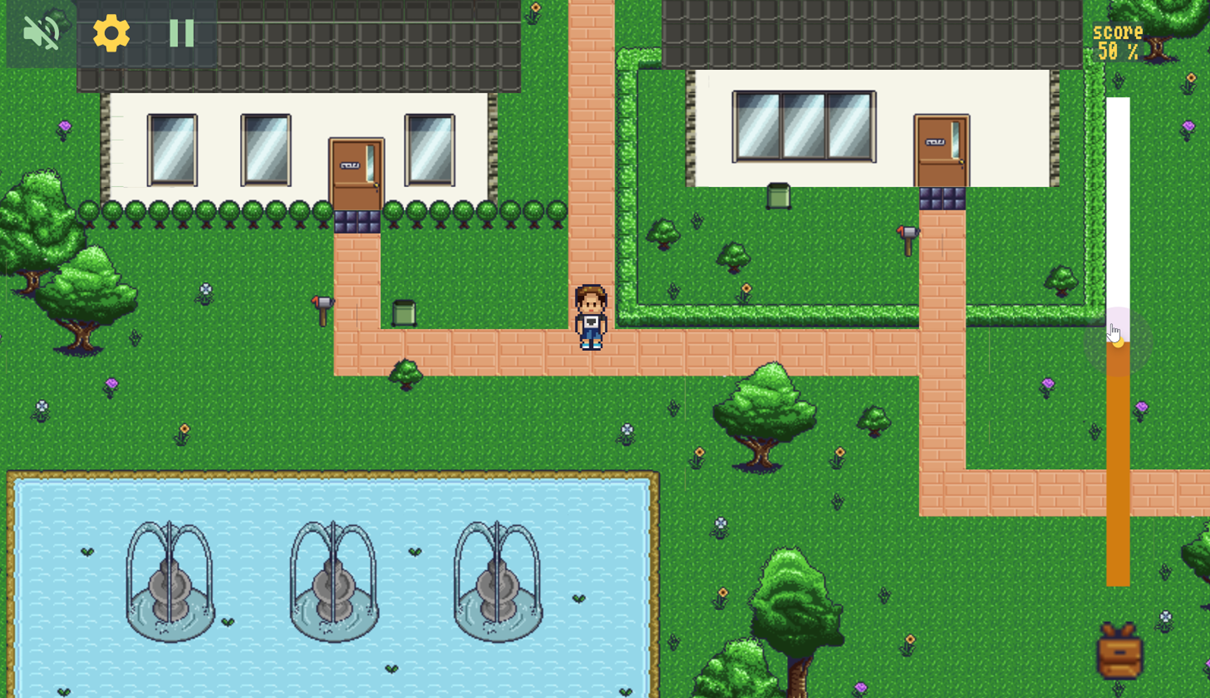
\includegraphics[width=0.8\textwidth ]{images/startingPage/village1.png}
    \caption{Village}
    \label{fig:pic_dessus}
\end{figure}

Dans le cas où l'utilisateur souhaiterait modifier les paramètres, il sera d'abord redirigé sur cette page avant de pouvoir lancer le jeu :
\begin{figure}[H]
    \centering
    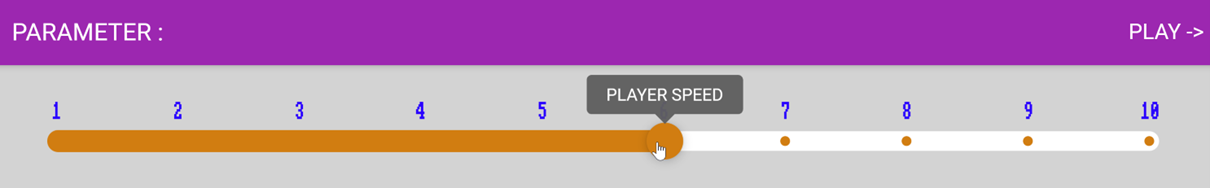
\includegraphics[width=0.8\textwidth ]{images/startingPage/setting.png}
    \caption{Paramètres}
    \label{fig:pic_dessus}
\end{figure}


%============================================================
%****************Les deplacements*******************

\subsection*{Les déplacements}
\addcontentsline{toc}{subsection}{Les deplacements}

Sur la carte, le joueur utilise les flèches du clavier pour se déplacer. Il peut aller dans quatre directions :

\begin{itemize}
    \item à droite:
          \begin{figure}[H]
              \centering
              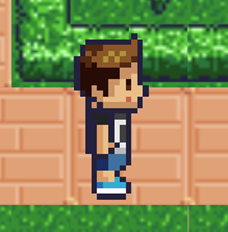
\includegraphics[width=0.1\textwidth ]{images/movements/playerRight.png}
              \caption{Mouvement du joueur à droite}
              \label{fig:pic_dessus}
          \end{figure}

    \item à gauche:
          \begin{figure}[H]
              \centering
              \includegraphics[width=0.1\textwidth ]{images/movements/playerLeft.png}
              \caption{Mouvement du joueur à gauche}
              \label{fig:pic_dessus}
          \end{figure}

    \item en bas:
          \begin{figure}[H]
              \centering
              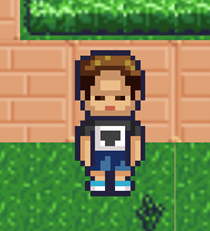
\includegraphics[width=0.1\textwidth ]{images/movements/playerDown.png}
              \caption{Mouvement du joueur en bas}
              \label{fig:pic_dessus}
          \end{figure}

    \item en haut:
          \begin{figure}[H]
              \centering
              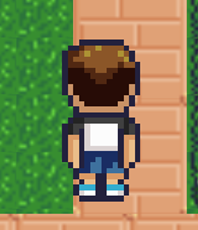
\includegraphics[width=0.1\textwidth ]{images/movements/playerUp.png}
              \caption{Mouvement du joueur en haut}
              \label{fig:pic_dessus}
          \end{figure}
\end{itemize}


Le joueur ne peut pas se déplacer partout! Lorsque qu'il rencontre un obstacle il est bloqué et ne peut pas passer par dessus.

%============================================================
%****************Le changement de scène*******************

\subsection*{Le changement de scène}
\addcontentsline{toc}{subsection}{Le changement de scène}

Maintenant que vous savez comment vous déplacer sur la carte, explorez-la ! Vous verrez qu'il est possible d'interagir avec des objets, des personnages.

Les joueurs peuvent par exemple entrer dans la maison de Mr. Moutarde en passant par la porte. Au moment où le joueur touche la porte, il entre dans la maison
\begin{figure}[H]
    \centering
    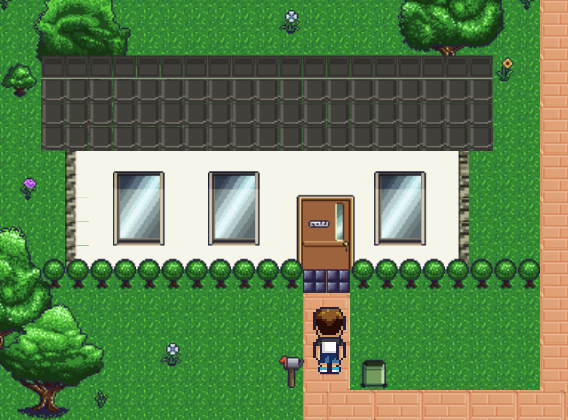
\includegraphics[width=0.8\textwidth ]{images/changeScene/changeSceneOut.png}
    \caption{Scène hors de la maison}
    \label{fig:pic_dessus}
\end{figure}

\begin{figure}[H]
    \centering
    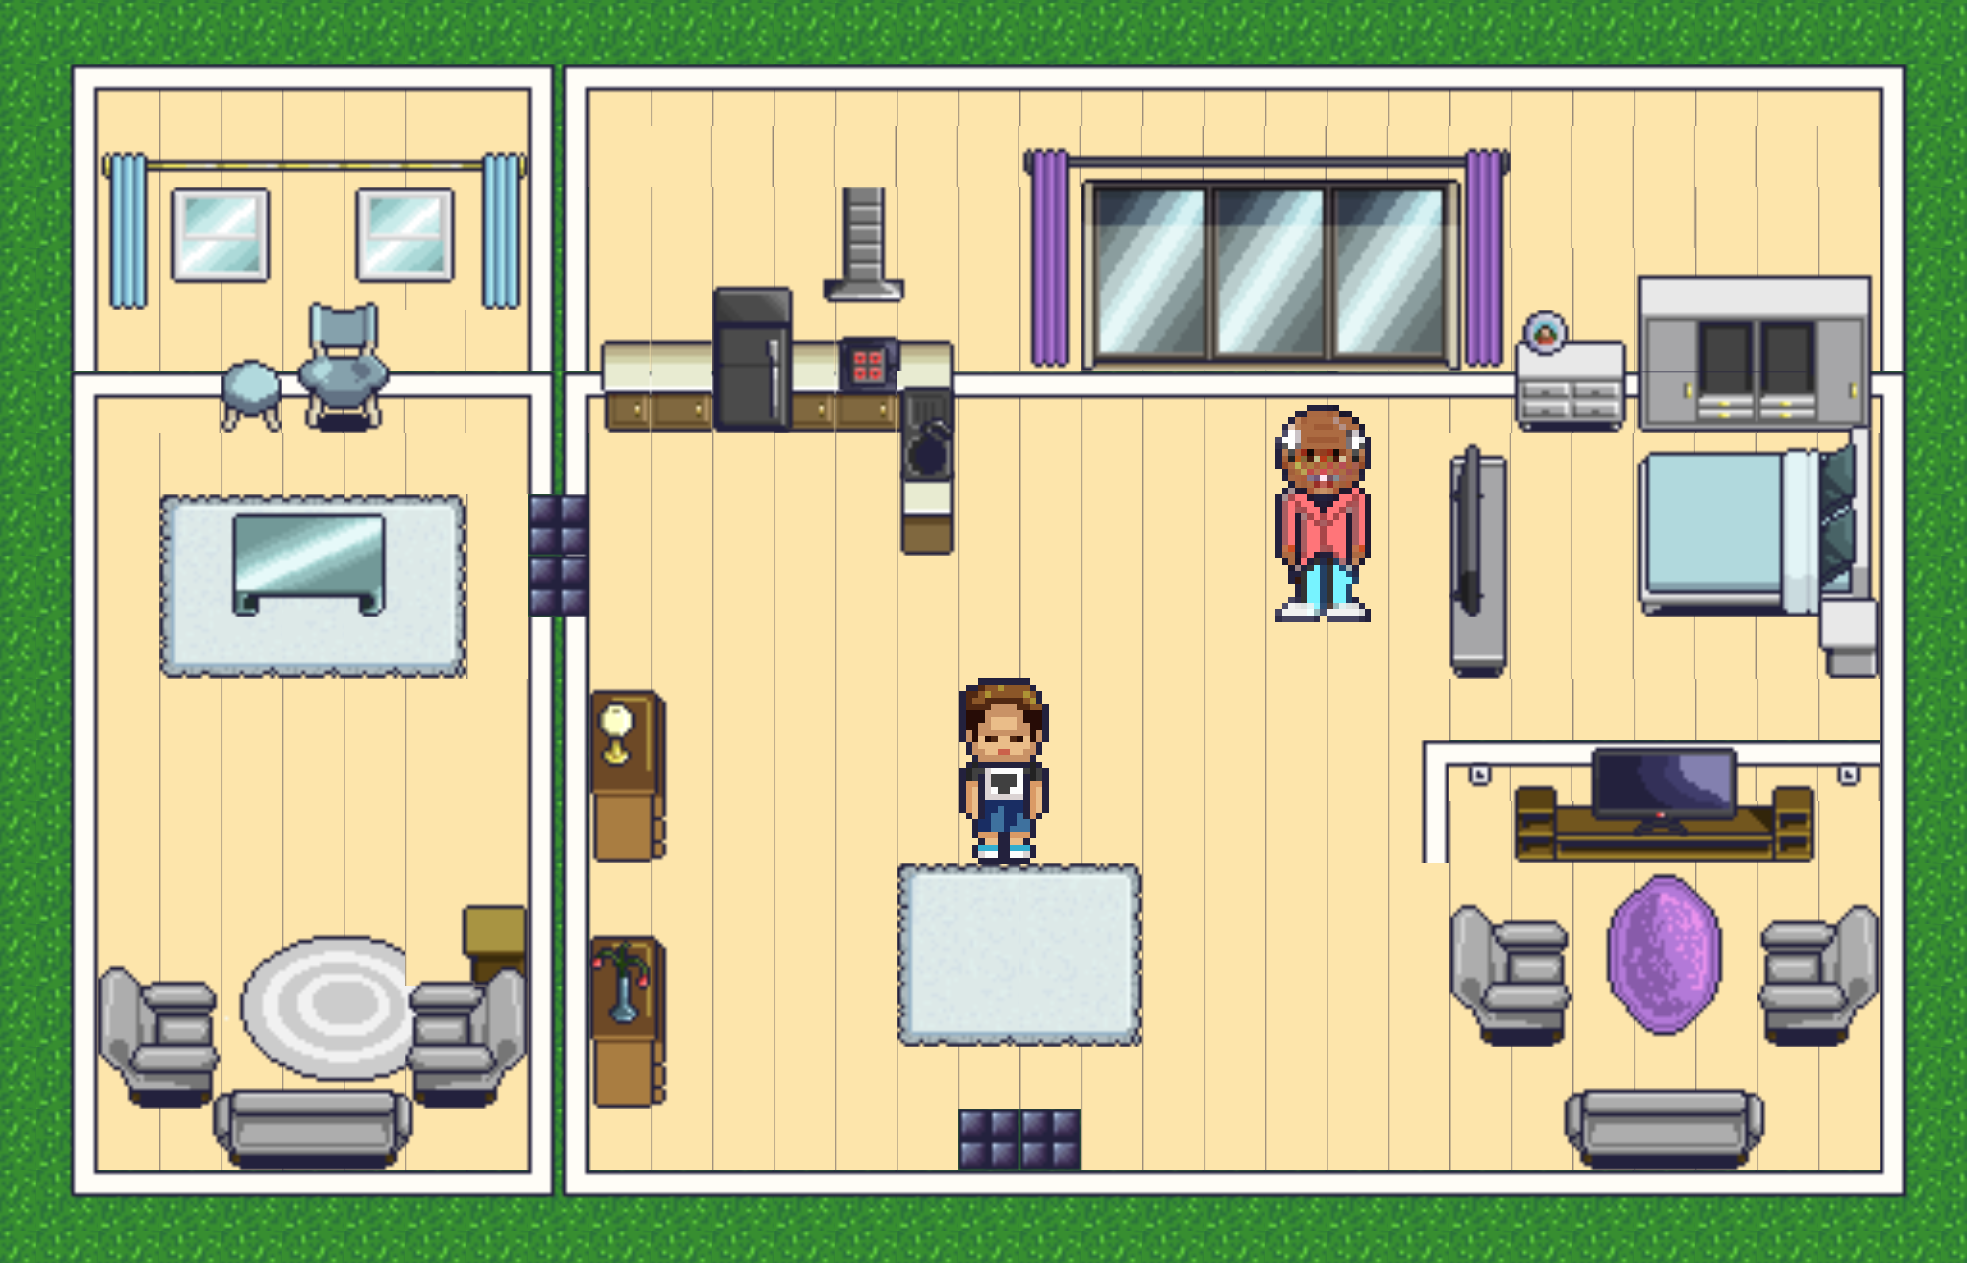
\includegraphics[width=0.8\textwidth ]{images/changeScene/changeSceneIn.png}
    \caption{Scène dans de la maison}
    \label{fig:pic_dessus}
\end{figure}

%============================================================
%****************Le dialogue*******************

\subsection*{Le dialogue}
\addcontentsline{toc}{subsection}{Le dialogue}

Le jeu intègre différents dialogues. Lorsque le joueur entre en collision avec certains personnages ou objets une boîte de dialogue apparaît. Par exemple, dans la maison de Mr. Moutarde, il est possible d'intéragir avec son propriétaire.
\begin{figure}[H]
    \centering
    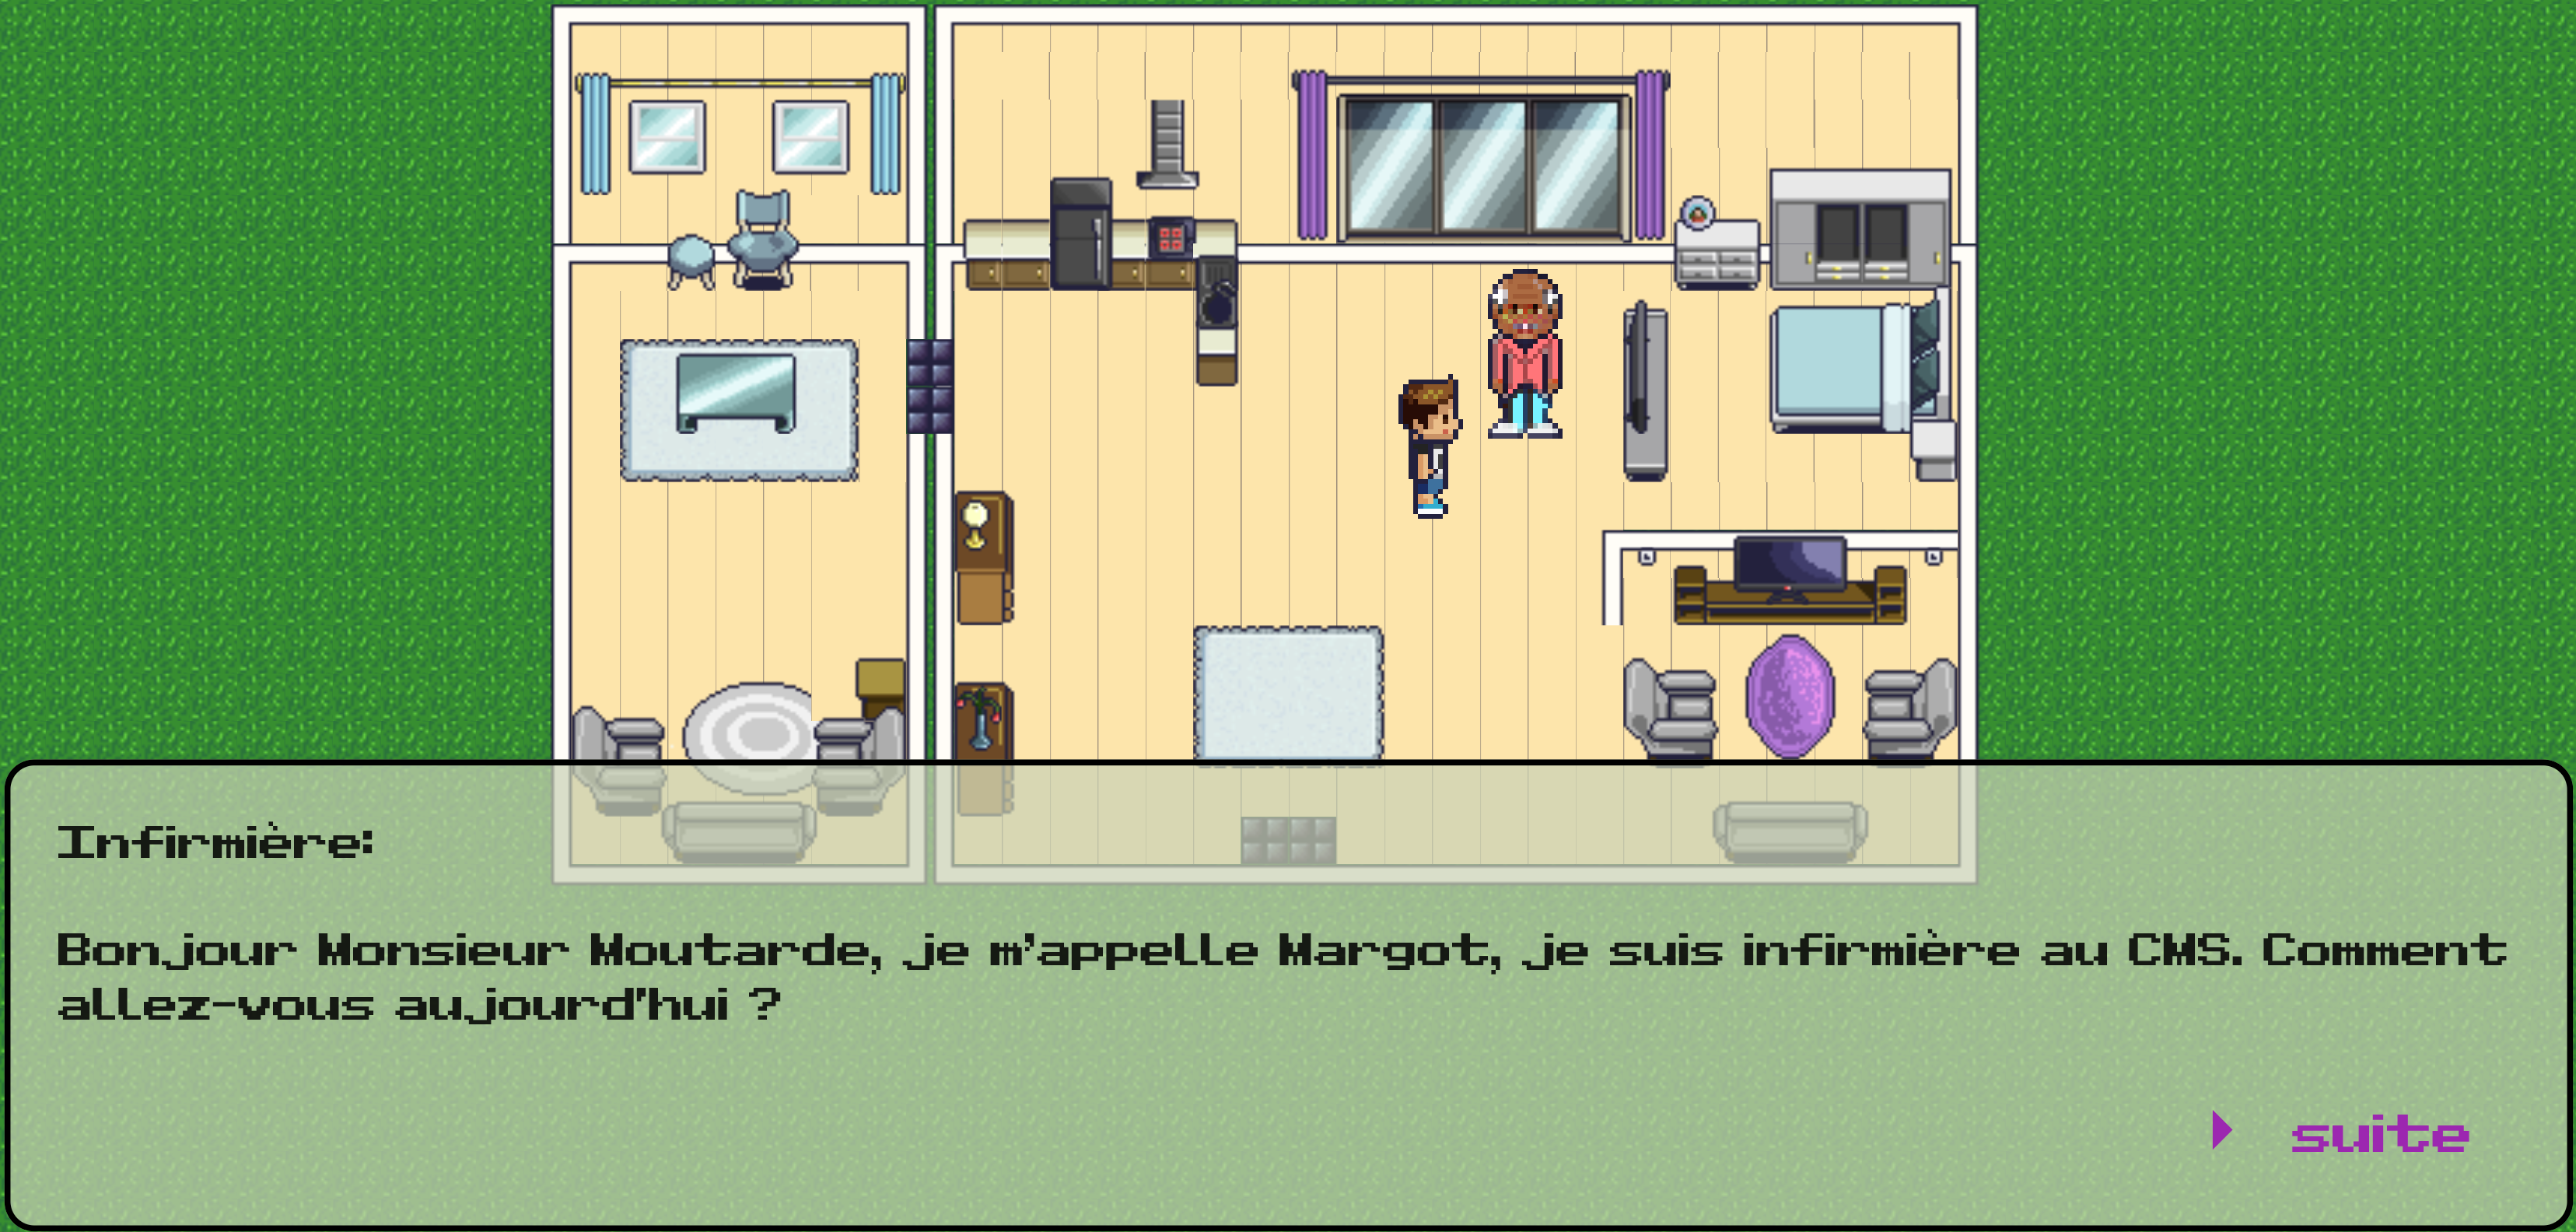
\includegraphics[width=0.8\textwidth ]{images/dialogs/dialog.png}
    \caption{Dialogue}
    \label{fig:pic_dessus}
\end{figure}

Certaines interactions peuvent demander une interaction de l'utilisateur. Si l'utilisateur réagit correctement, il peut gagner des points et bien sûr, s'il réagit de la mauvaise des manières, il en perd. La plupart du temps, en cas de mauvaise réponse, le joueur a le possibilité d'en choisir une autre sans qu'elle ne lui fasse perdre ou gagner d'autres points.

Voici les différents types de dialogue utilisés :
\begin{figure}[H]
    \centering
    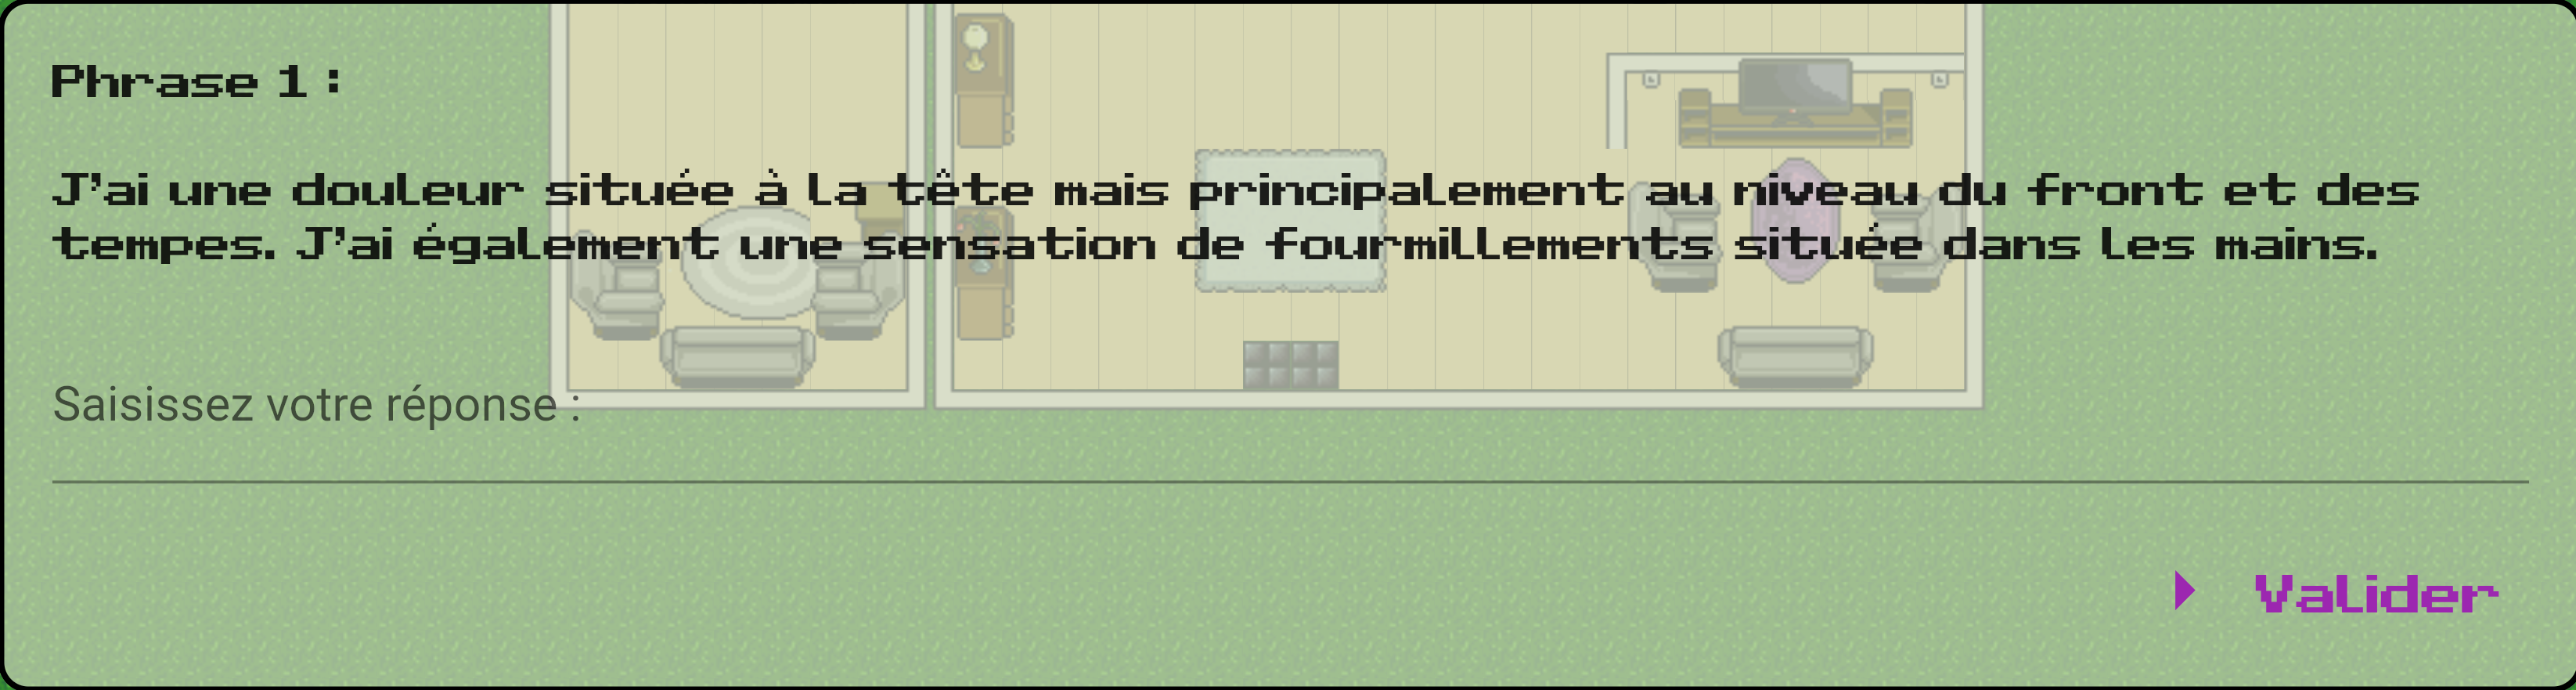
\includegraphics[width=0.8\textwidth ]{images/dialogs/dialogInput.png}
    \caption{Dialogue - Réponse libre}
    \label{fig:pic_dessus}
\end{figure}

\begin{figure}[H]
    \centering
    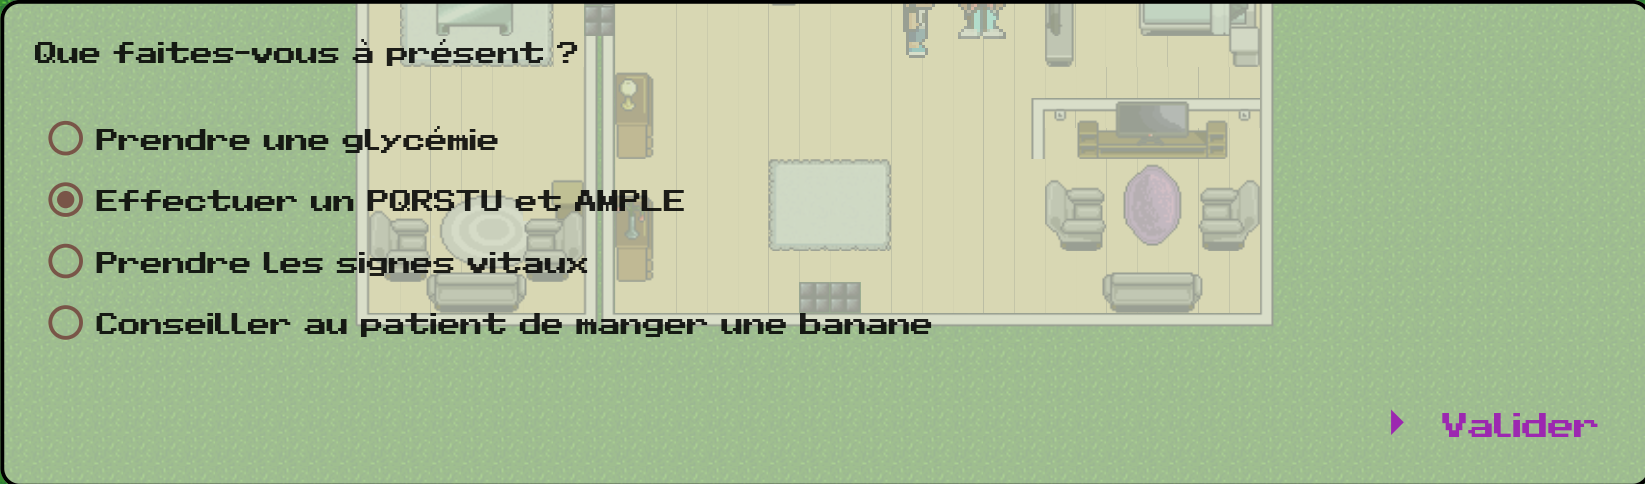
\includegraphics[width=0.8\textwidth ]{images/dialogs/dialogRadioButton.png}
    \caption{Dialogue - Choix unique}
    \label{fig:pic_dessus}
\end{figure}

\begin{figure}[H]
    \centering
    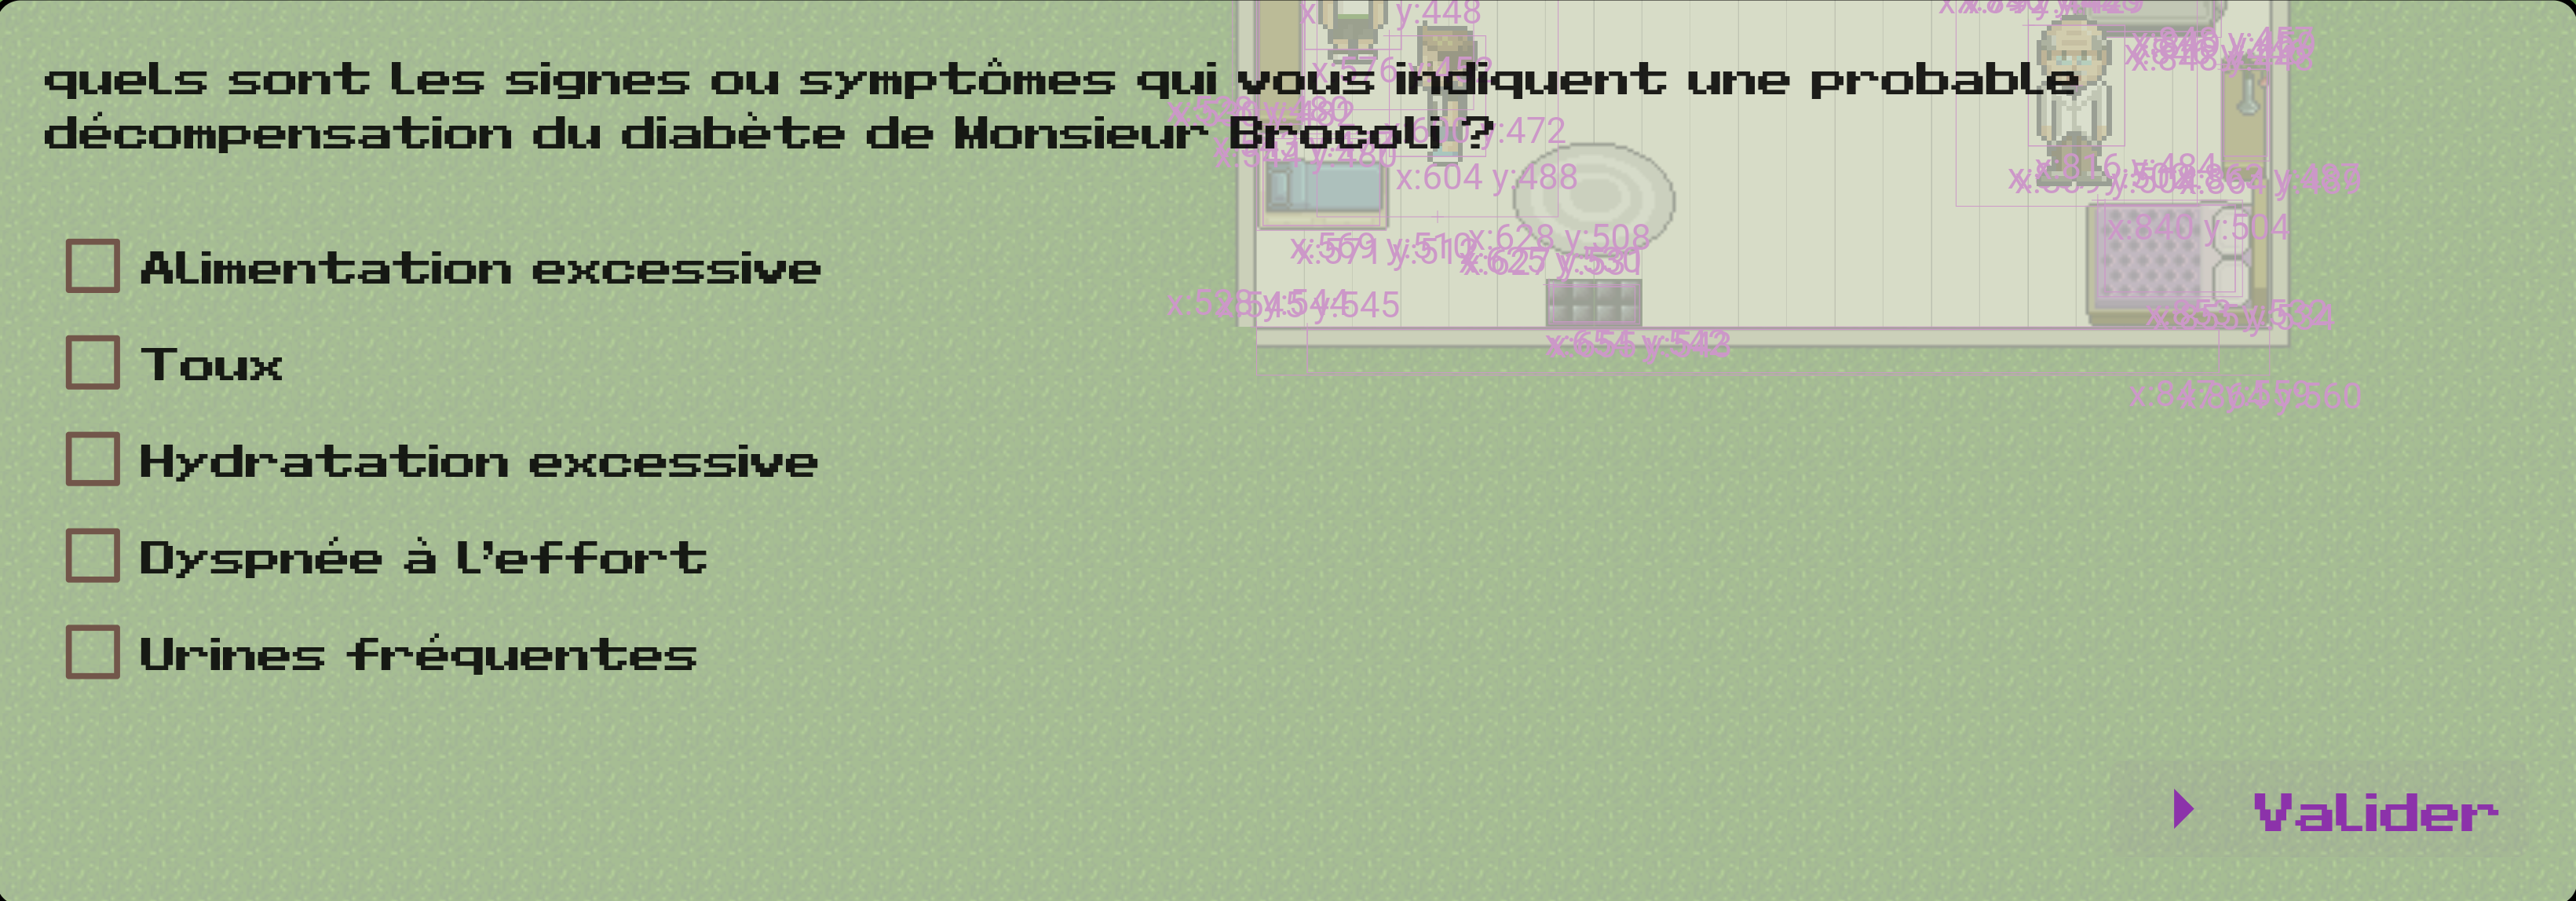
\includegraphics[width=0.8\textwidth ]{images/dialogs/dialogCheckbox.png}
    \caption{Dialogue - Choix multiple}
    \label{fig:pic_dessus}
\end{figure}


%============================================================
%****************Le score*******************

\subsection*{Le score}
\addcontentsline{toc}{subsection}{Le score}

À droite de l'écran, une barre verticale est affichée. Elle représente le score du joueur. L'utilisateur commence le jeu avec 50 points. Durant les différentes situations, le joueur pourra gagner ou perdre des points.

Plus l'utilisateur a de points, plus la jauge affichant le score se remplira et inversement. La barre du score change de couleur selon les points du joueur. Le vert signifiant un bon score et le rouge un mauvais.
\begin{figure}[H]
    \centering
    \includegraphics[height=0.4\textheight ]{images/score.png}
    \caption{Score}
    \label{fig:pic_dessus}
\end{figure} 



%============================================================
%****************Sac à dos*******************

\subsection*{Le sac à dos}
\addcontentsline{toc}{subsection}{Le sac à dos}

L'utilisateur a la possibilité d'afficher le contenu du sac à dos en cliquant sur l'icône sac en bas à droite de l'écran.

\begin{figure}[H]
    \centering
    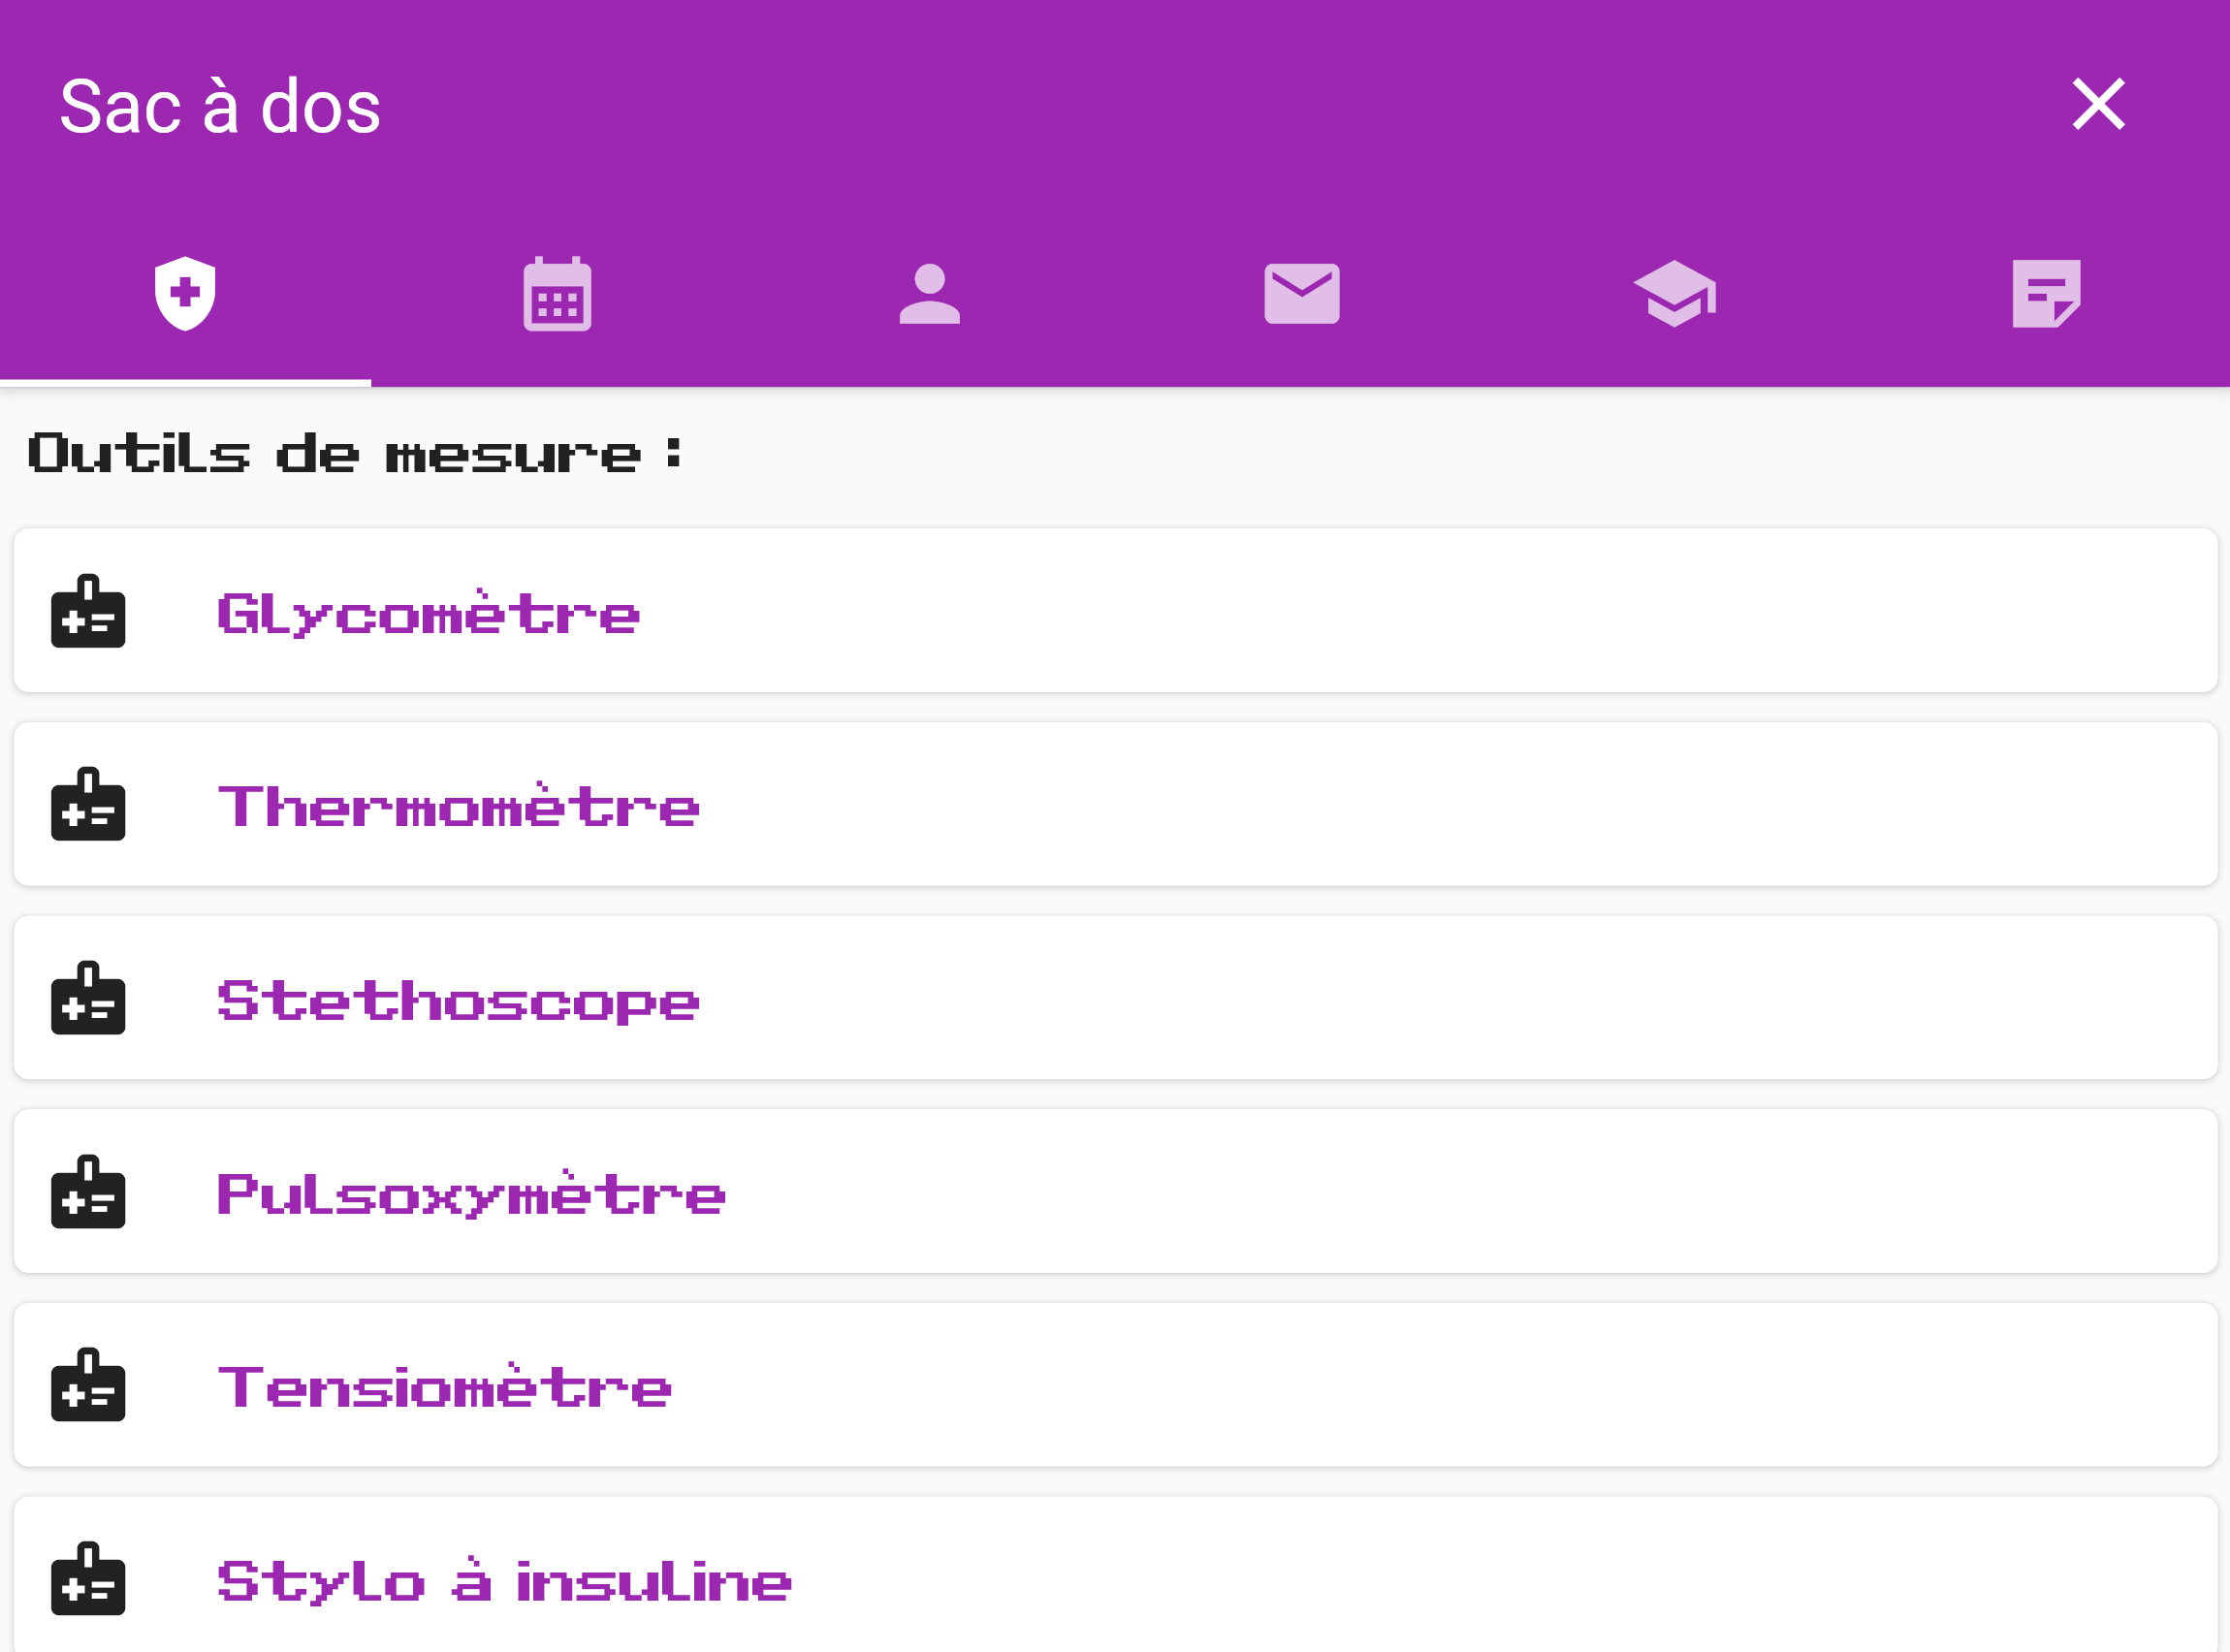
\includegraphics[width=0.8\textwidth ]{images/toolsMenu/toolbox.png}
    \caption{Sac à dos}
    \label{fig:pic_dessus}
\end{figure}

Le sac à dos contient les onglets suivants:
\begin{itemize}
    \item les outils de mesure
    \item le planning de la journée
    \item les situations des patients
    \item la liste de professionnels
    \item la collection des apprentissages
    \item les notes sur les patients
\end{itemize}

%============================================================
%****************Onglet 1 outils*******************

\subsubsection*{Outils de mesure}
\addcontentsline{toc}{subsubsection}{Outils de mesure}

Le premier onglet du menu du sac à dos contient les différents outils de mesure. En cliquant sur cet onglet, l'utilisateur a la possibilité de sélectionner les outils à opérer sur les patients. \\

\begin{figure}[H]
    \centering
    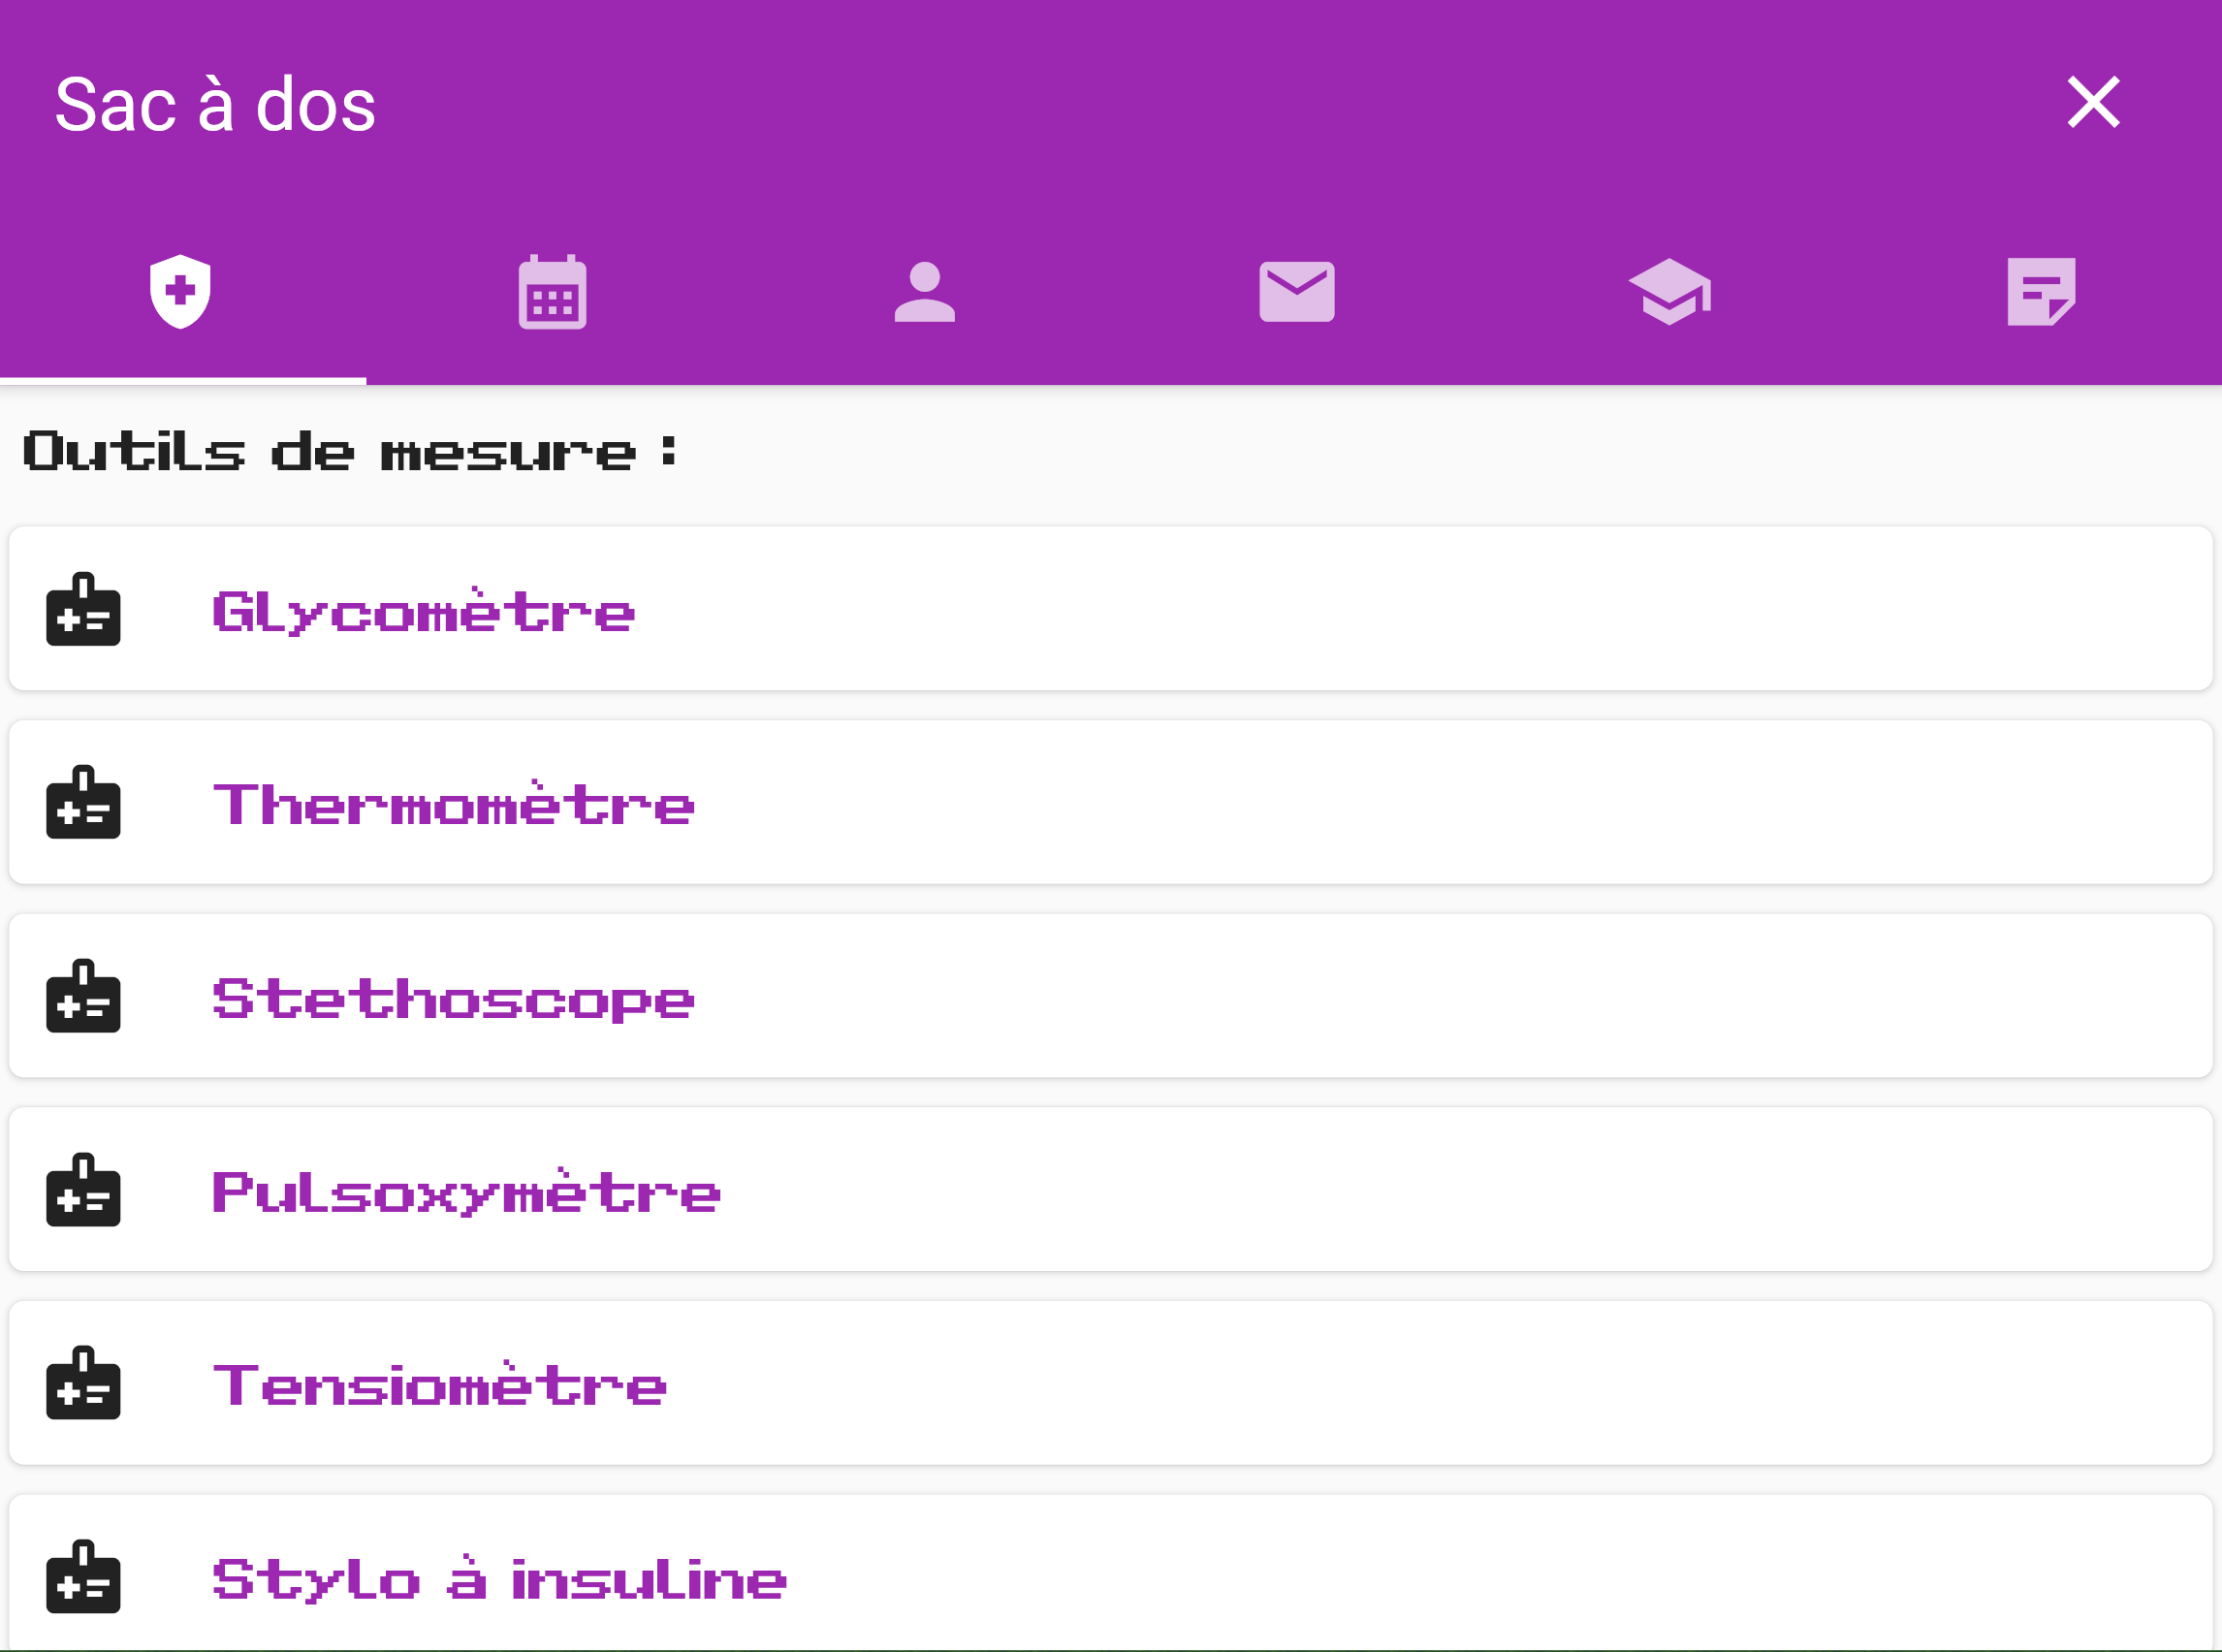
\includegraphics[width=0.8\textwidth ]{images/toolsMenu/tools.png}
    \caption{Sac à dos - Outils de mesure}
    \label{fig:pic_dessus}
\end{figure}

Lorsque nous cliquons sur un outil qui ne peut pas être utilisé, un dialogue nous en avertit.

\begin{figure}[H]
    \centering
    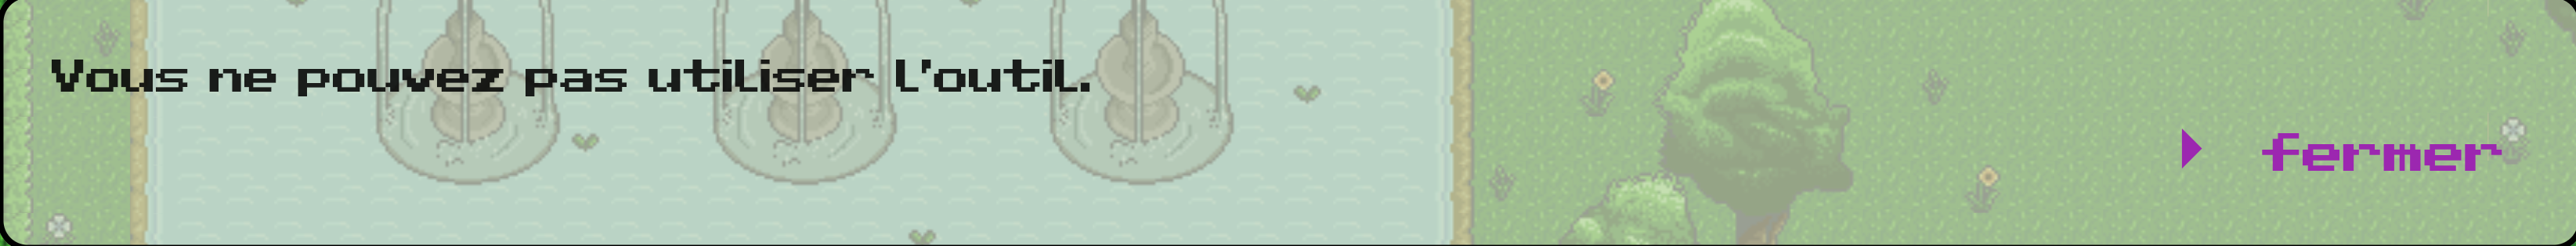
\includegraphics[width=0.8\textwidth ]{images/toolsMenu/toolCantBeUsed.png}
    \caption{Sac à dos - Outils de mesure ne peut être utilisé}
    \label{fig:pic_dessus}
\end{figure}

En revanche, lorsqu'un outil est utilisable, un dialogue indique la mesure prise.
\begin{figure}[H]
    \centering
    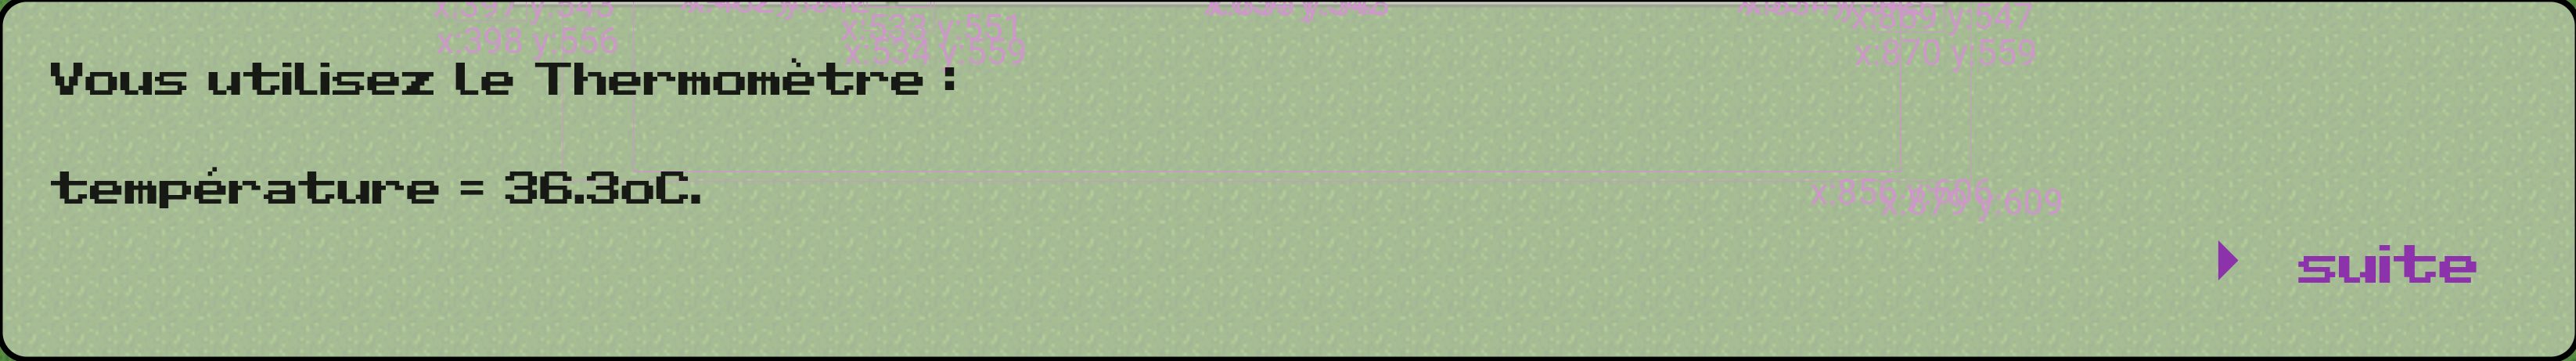
\includegraphics[width=0.8\textwidth ]{images/toolsMenu/toolCanBeUsed.png}
    \caption{Sac à dos - Outils de mesure utilisé}
    \label{fig:pic_dessus}
\end{figure}

%============================================================
%****************Onglet 2 planning*******************

\subsubsection*{Planning de la journée}
\addcontentsline{toc}{subsubsection}{Planning de la journée}

Le second onglet du menu du sac à dos est le planning. En cliquant sur cet onglet, l'utilisateur a la possibilité de visualiser son planning de la journée. \\

\begin{figure}[H]
    \centering
    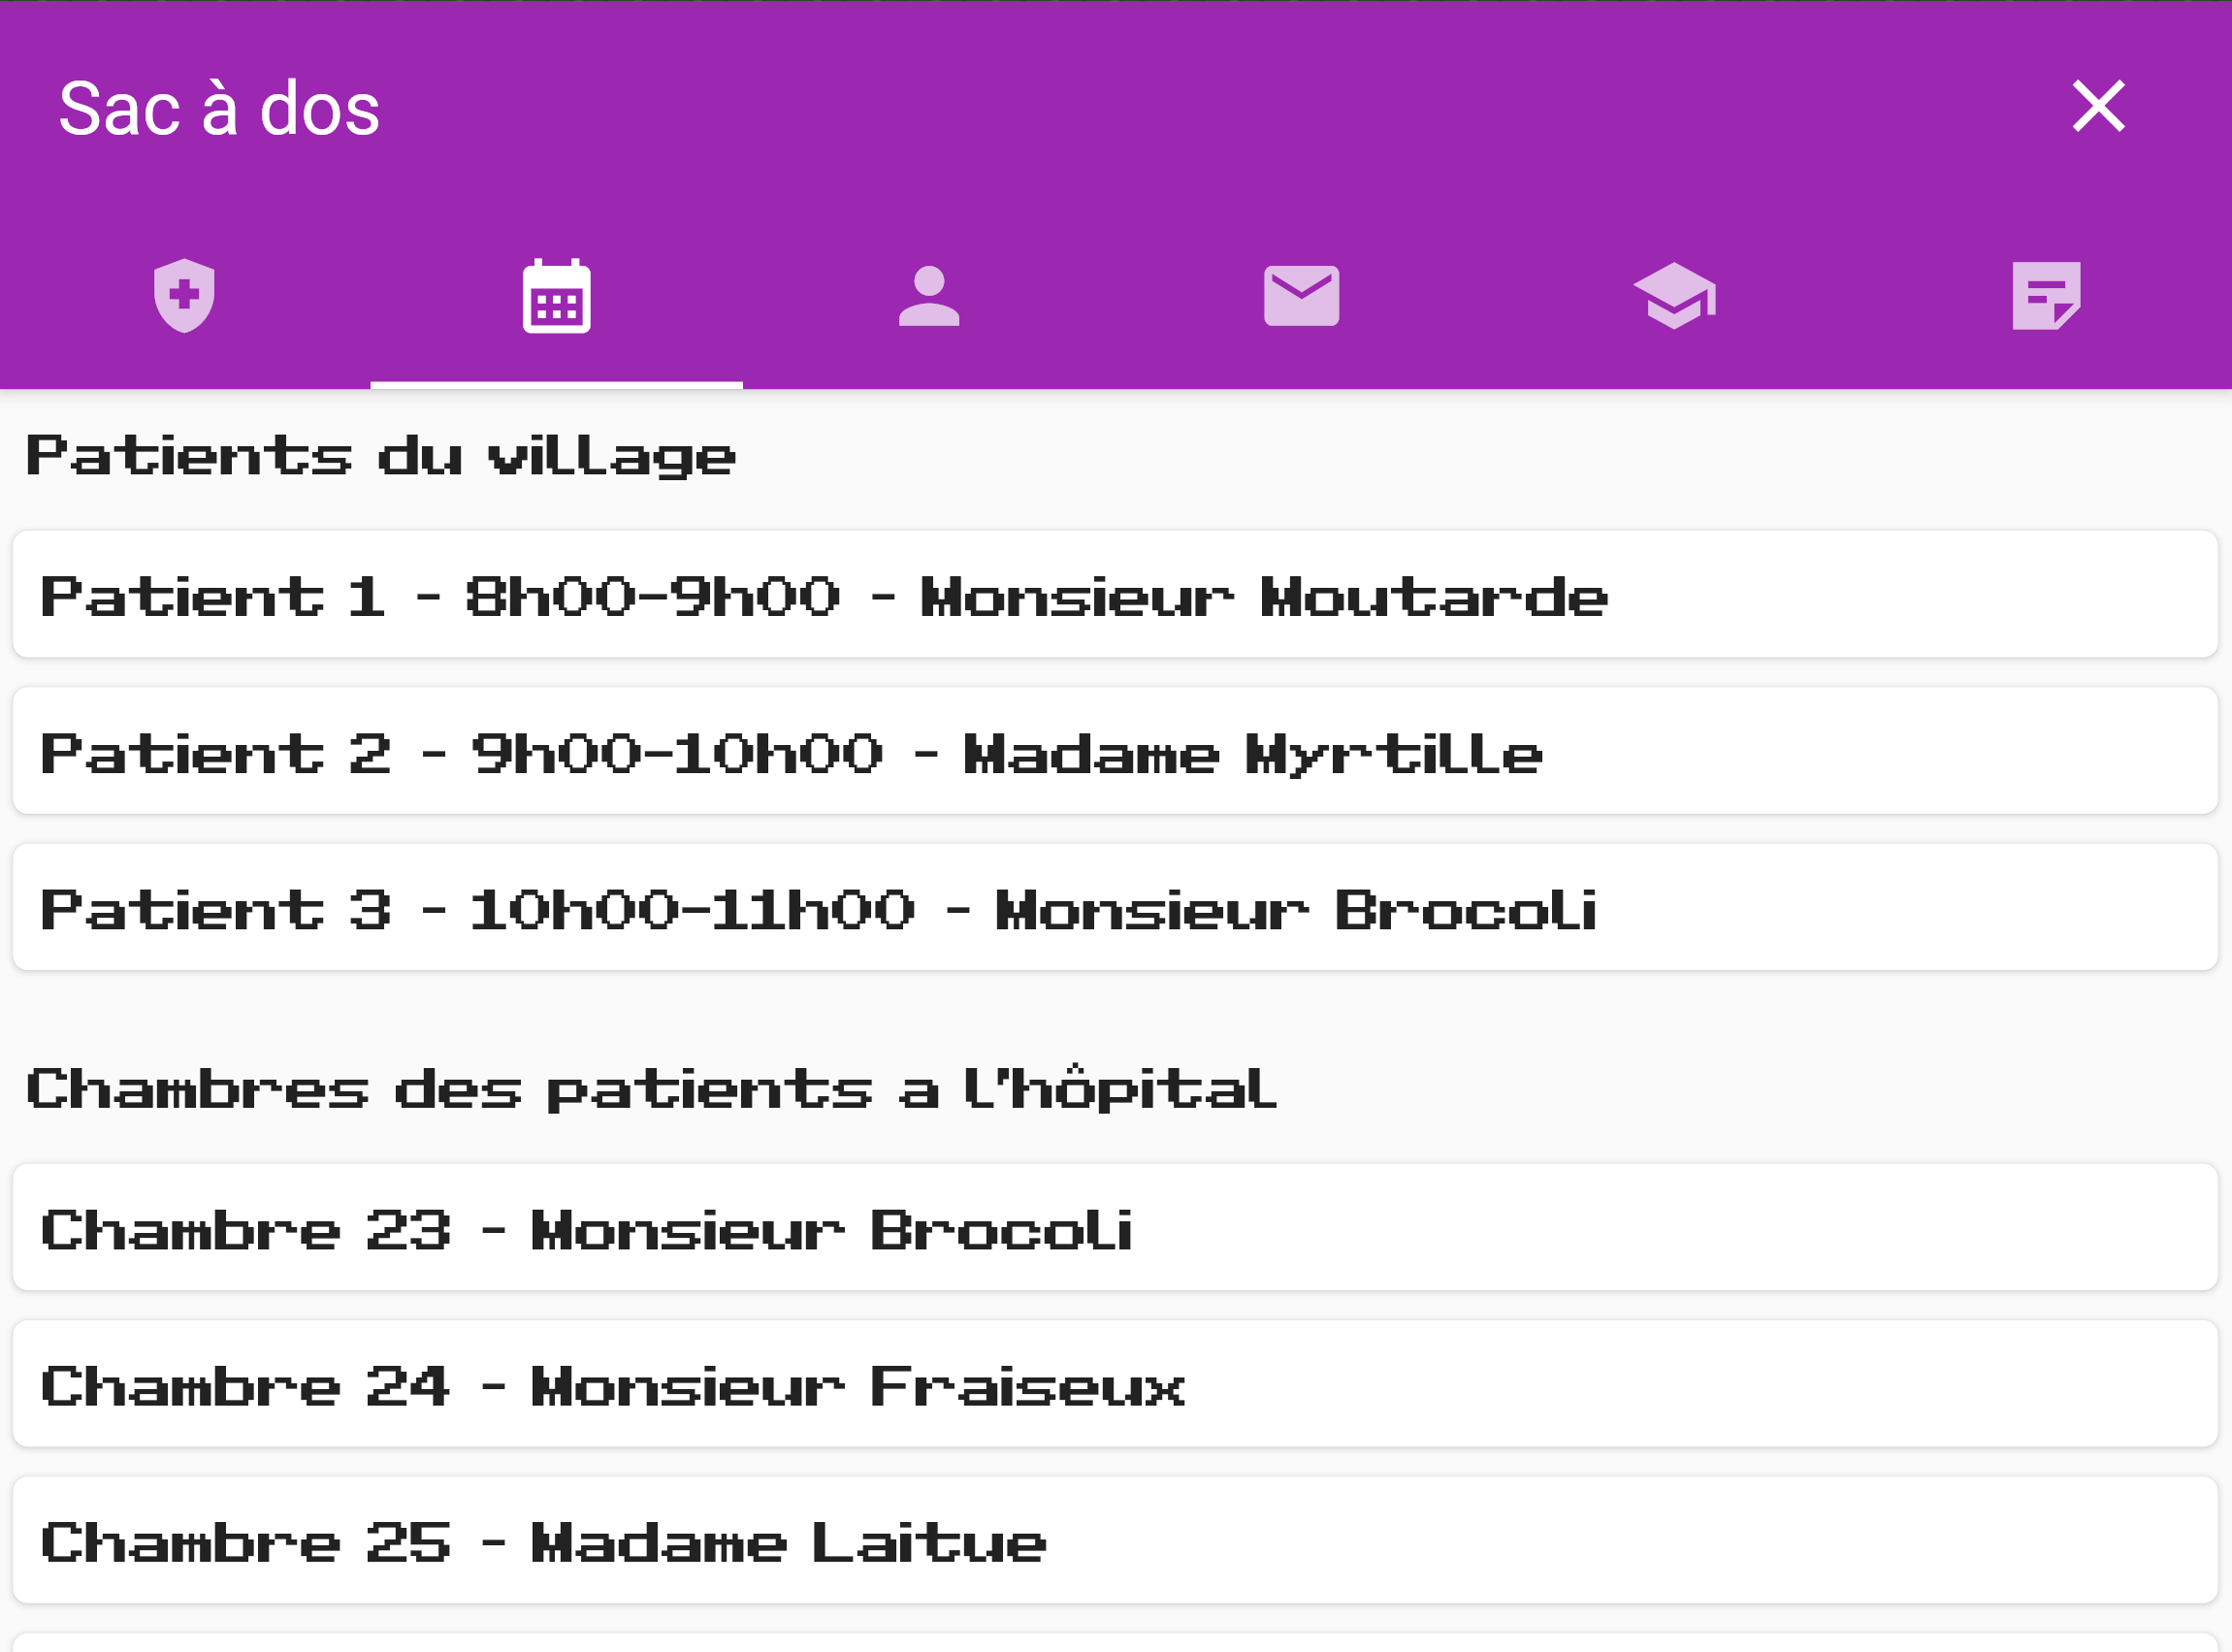
\includegraphics[width=0.8\textwidth ]{images/toolsMenu/planning.png}
    \caption{Sac à dos - Planning de la journée}
    \label{fig:pic_dessus}
\end{figure}

%============================================================
%****************Onglet 3 Situation des patiens*******************

\subsubsection*{Situation des patients}
\addcontentsline{toc}{subsubsection}{Situation des patients}

Le troisième onglet du menu du sac à dos est la situation des patients. En cliquant sur cet onglet, l'utilisateur a la possibilité de visualiser la situation des différents patients à consulter. \\

\begin{figure}[H]
    \centering
    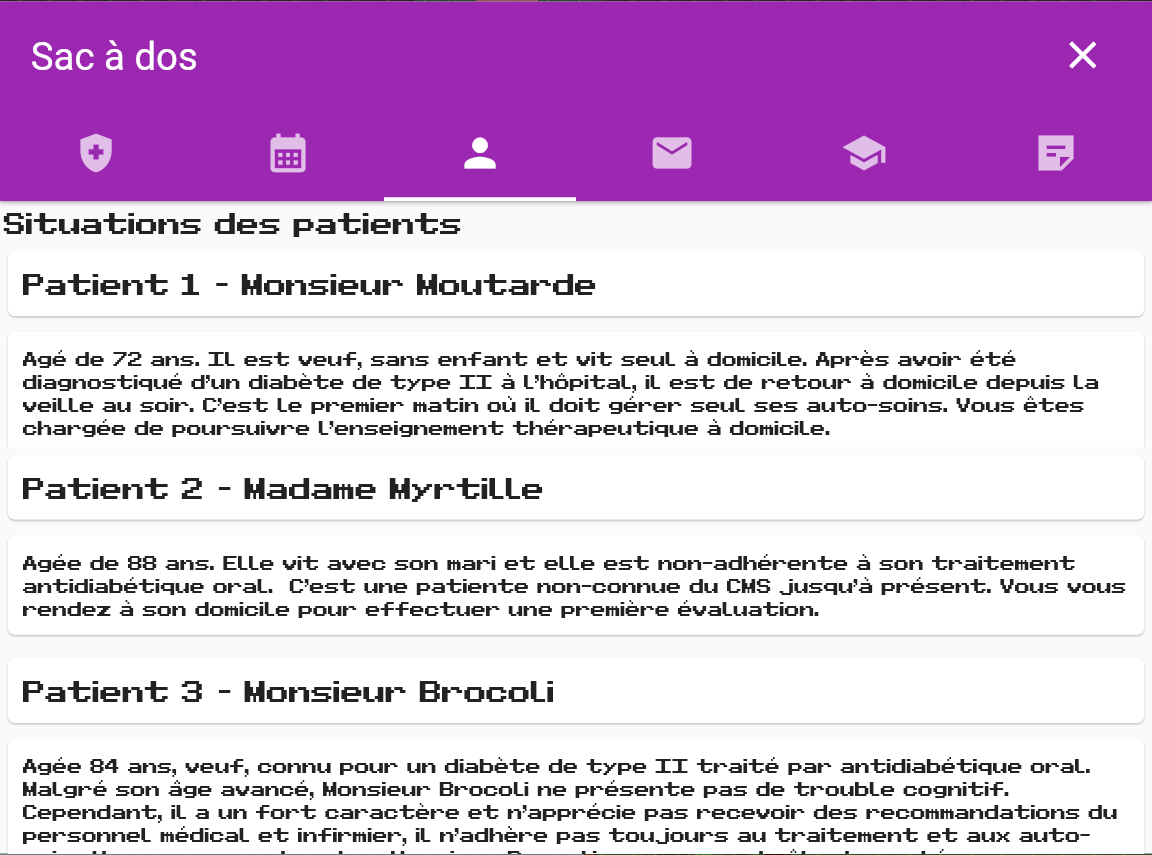
\includegraphics[width=0.8\textwidth ]{images/toolsMenu/situations.png}
    \caption{Sac à dos - Situations des patients}
    \label{fig:pic_dessus}
\end{figure}

%============================================================
%****************Onglet 4 Contacts*******************

\subsubsection*{Contacts}
\addcontentsline{toc}{subsubsection}{Contacts}

Le quatrième onglet du menu du sac à dos contient les contacts. En cliquant sur cet onglet, l'utilisateur a la possibilité de contacter différentes personnes au cours de son jeu. \\

\begin{figure}[H]
    \centering
    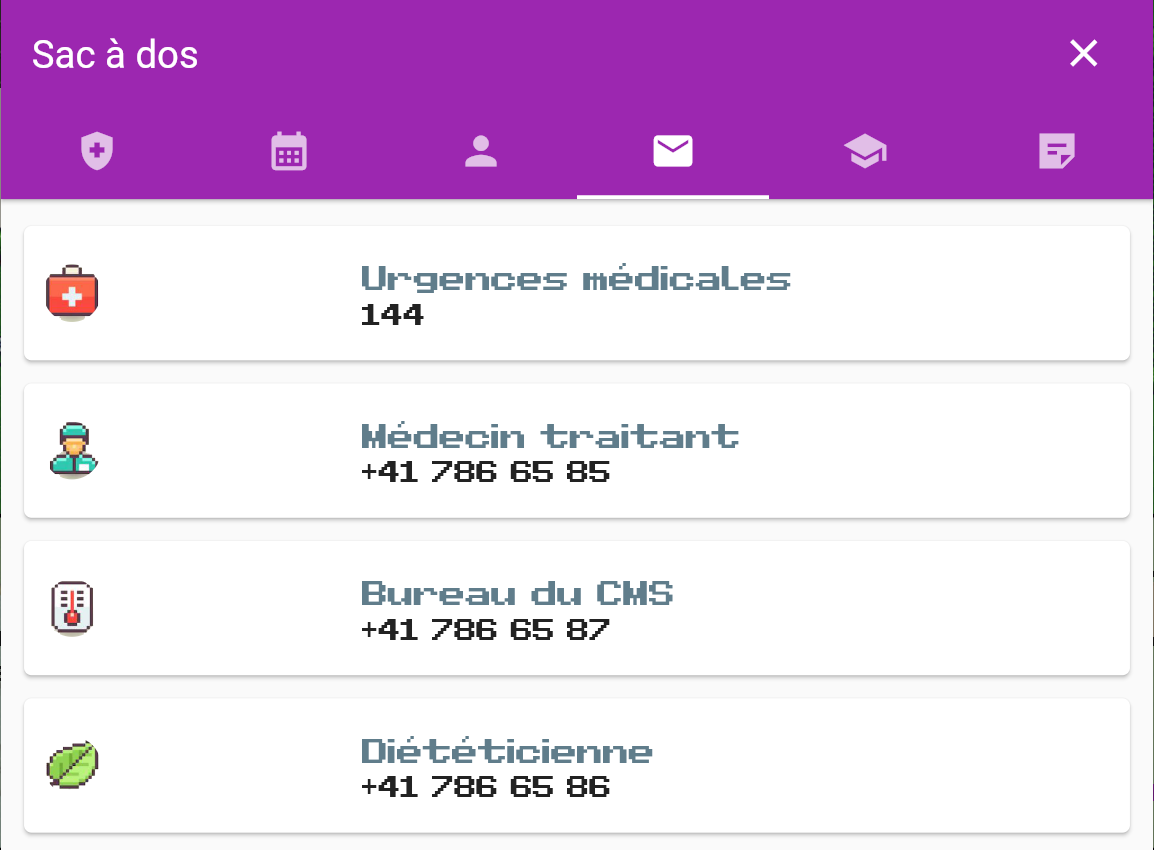
\includegraphics[width=0.8\textwidth ]{images/toolsMenu/contacts.png}
    \caption{Sac à dos - Contacts}
    \label{fig:pic_dessus}
\end{figure}

En cliquant sur un contact alors qu'il n'en a pas l'utilité, un dialogue s'affiche.
\begin{figure}[H]
    \centering
    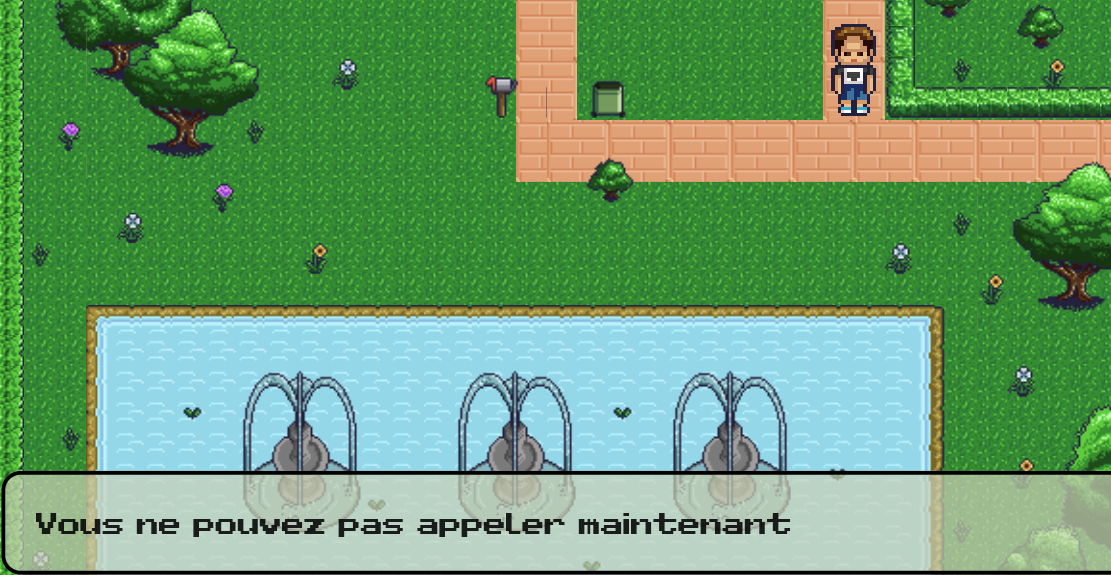
\includegraphics[width=0.8\textwidth ]{images/toolsMenu/contactCantBeUsed.png}
    \caption{Sac à dos - Contact ne peut être appelé}
    \label{fig:pic_dessus}
\end{figure}

En revanche, lorsqu'un contact peut être atteint, un dialogue vous l'indique.
\begin{figure}[H]
    \centering
    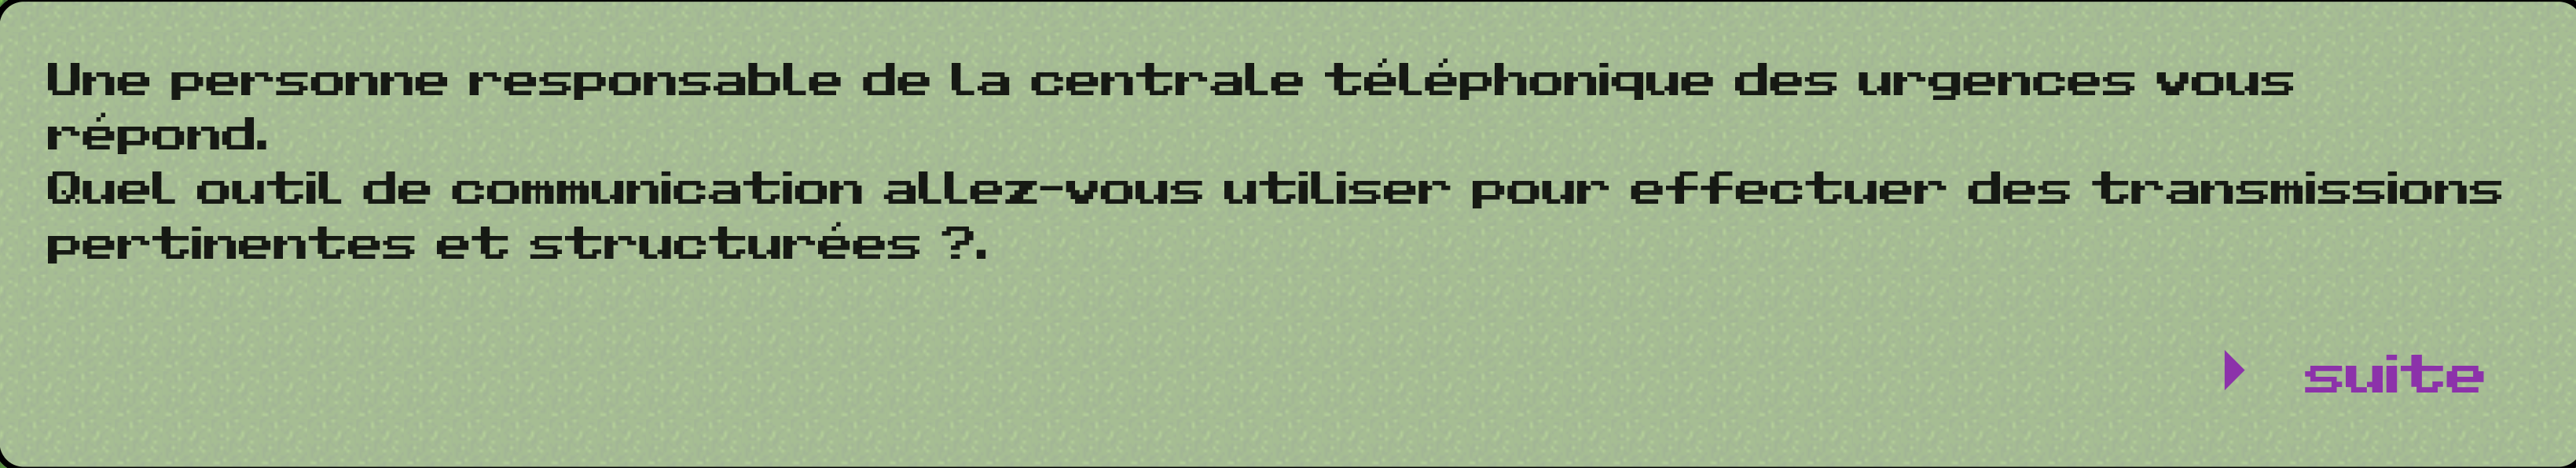
\includegraphics[width=0.8\textwidth ]{images/toolsMenu/contactCanBeUsed.png}
    \caption{Sac à dos - Contact appelé}
    \label{fig:pic_dessus}
\end{figure}

%============================================================
%****************Onglet 5 Collection d'apprentissage*******************

\subsubsection*{Collection d'apprentissage}
\addcontentsline{toc}{subsubsection}{Collection d'apprentissage}

Le cinquième onglet du menu du sac à dos contient les collections d'apprentissage. En cliquant sur cet onglet, l'utilisateur a la possibilité de visualiser les différentes collections d'apprentissage qui lui seront décernées au cours du jeu. \\

\begin{figure}[H]
    \centering
    
\includegraphics[width=0.8\textwidth ]{images/toolsMenu/collections.png}
    \caption{Sac à dos - Collections}
    \label{fig:pic_dessus}
\end{figure}

%============================================================
%****************Onglet 6 Notes*******************

\subsubsection*{Notes}
\addcontentsline{toc}{subsubsection}{Notes}

Le sixième onglet du menu du sac à dos contient les notes. En cliquant sur cet onglet, l'utilisateur a la possibilité de visualiser les différentes notes des patients qu'il aura visités au cours du jeu. \\

\begin{figure}[H]
    \centering
    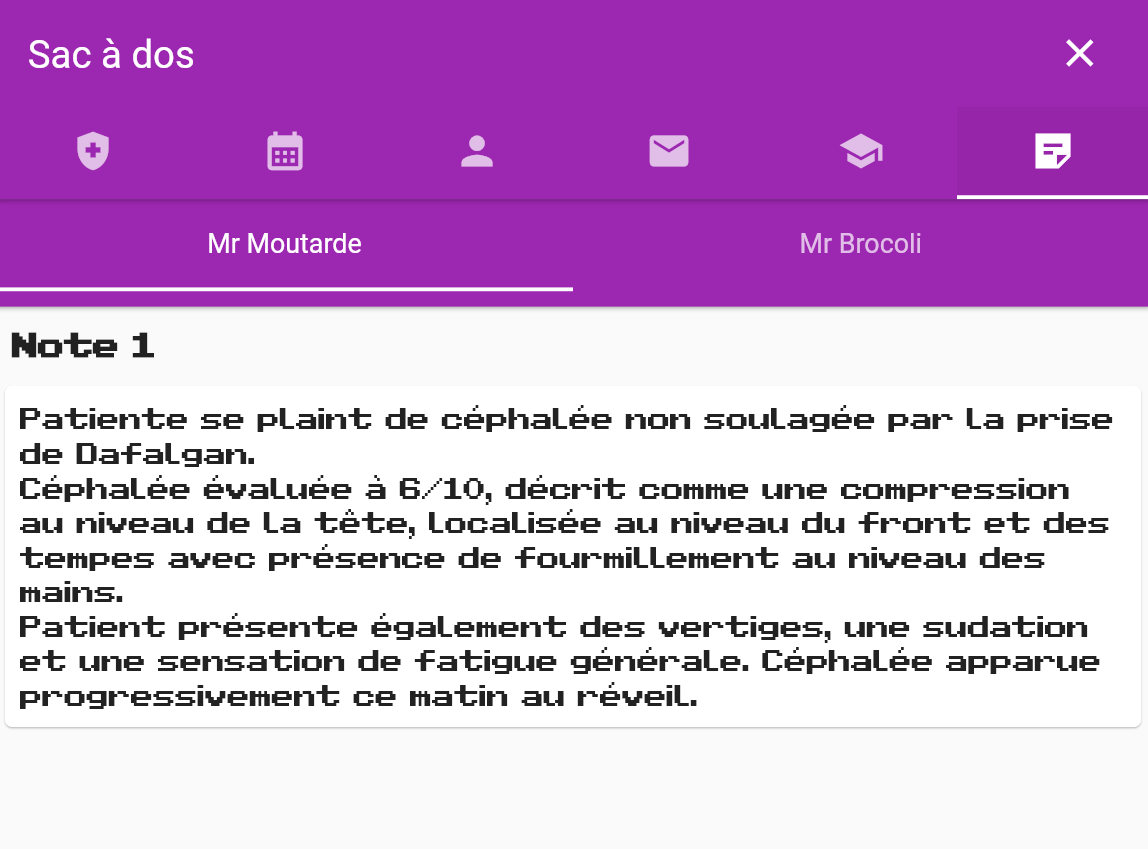
\includegraphics[width=0.8\textwidth ]{images/toolsMenu/notes.png}
    \caption{Sac à dos - Notes}
    \label{fig:pic_dessus}
\end{figure}


%============================================================
%****************Bonnes pratiques*******************

\subsection*{Bonnes pratiques}
\addcontentsline{toc}{subsection}{Bonnes pratiques}

Afin de pouvoir jouer correctement au jeu, voici quelques conseils :
\begin{itemize}
    \item Utilisez le navigateur Chrome avec la dernière version.
    \item Appuyez sur 1 des touches de déplacements (flèches) à la fois.
    \item Attendez la fin des dialogues avant d'appuyer sur d'autres touches.
    \item Si un obstacle bloque le passage, il faut le contourner.
    \item Terminez la mission avant de se diriger vers la sortie. Actuellement il y a une alerte si la mission n'est pas terminée.
    \item Il n'est pas possible de re-effectuer une mission déjà réalisée.
    \item Afin de valider une réponse à une question à libre choix, il est possible d'appuyer sur la toucher Enter.
    \item Evitez de sortir de l'enceinte des bâtiments au risque de ne plus pouvoir revenir à l'intérieur.
\end{itemize}

En cas de problème tel qu'un problème d'affichage ou impossibilité de se déplacer, veuillez essayer cliquer sur la touche tabulation. Si cette dernière ne règle pas le problème, raffraichissez la page pour recommencer le jeu.

\end{document}
